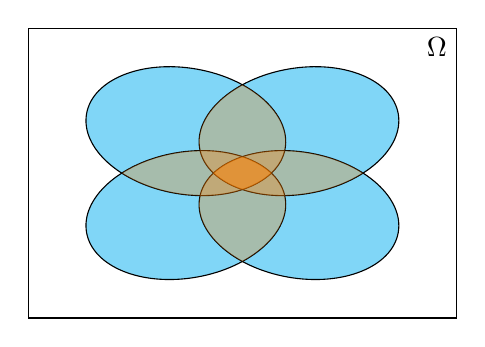
\begin{tikzpicture}[scale=1.6]

    \draw (-.2,-.2) rectangle (3.2,2.1);
    \node [below left] at (3.2,2.1) {$\Omega$};

    \def\circleOne{[
        rotate around={10:(1.5,0.95)},
        xshift=-.5cm,
        yshift=-.25cm,
    ] (1.5,0.95) ellipse (.8 and .5)}
    \def\circleTwo{[
        rotate around={10:(1.5,0.95)},
        xshift=.5cm,
        yshift=.25cm,
    ] (1.5,0.95) ellipse (.8 and .5)}
    \def\circleThree{[
        rotate around={-10:(1.5,0.95)},
        xshift=.5cm,
        yshift=-.25cm,
    ] (1.5,0.95) ellipse (.8 and .5)}
    \def\circleFour{[
        rotate around={-10:(1.5,0.95)},
        xshift=-.5cm,
        yshift=.25cm,
    ] (1.5,0.95) ellipse (.8 and .5)}

    \fill[cyan!50] \circleOne;
    \fill[cyan!50] \circleTwo;
    \fill[cyan!50] \circleThree;
    \fill[cyan!50] \circleFour;

    \draw \circleOne;
    \draw \circleTwo;
    \draw \circleThree;
    \draw \circleFour;

    \begin{scope}
        \clip \circleOne;
        \fill[orange,fill opacity=.3] \circleFour;
    \end{scope}
    \begin{scope}
        \clip \circleTwo;
        \fill[orange,fill opacity=.3] \circleThree;
    \end{scope}
    \begin{scope}
        \clip \circleOne;
        \fill[orange,fill opacity=.3] \circleThree;
    \end{scope}
    \begin{scope}
        \clip \circleTwo;
        \fill[orange,fill opacity=.3] \circleFour;
    \end{scope}

\end{tikzpicture}